
\chapter{A generic sound processing library}

\epigraph{Numbers it is. All music when you come to think.  Two
  multiplied by two divided by half is twice one.  Vibrations: chords
  those are. One plus two plus six is seven. Do anything you like with
  figures juggling. Always find out this equal to that. Symmetry under
  a cemetery wall. He doesn’t see my mourning. Callous: all for his
  own gut. Musemathematics. And you think you’re listening to the
  etherial. But suppose you said it like: Martha, seven times nine
  minus $x$ is thirtyfive thousand.  Fall quite flat. It’s on account of
  the sounds it is.}{\emph{Ulysses}\\\textsc{James Joyce}}

\section{Analysis}

Requirements \ref{req:iter1-begin} to \ref{req:iter1-end} and
\ref{req:iter1-begin2} to \ref{req:iter1-end2} refer to the second
layer of our system --- in a bottom-up approach. The most crucial
question here: how do we represent a sound in a computer? Then, a new
question arises: how do we get the sound to the speakers? The later
question has a trivial answer --- use whatever API your operating
system exposes for delivering sound to the soundcard --- but the first
question is still to be answered. Actually, the solution to this first
question mostly subsumes the issue of how to interface with these
external interfaces, thus, shall we debate it with care.

\subsection{Factors of sound representation}
\todo{Me he dado cuenta de que esta sección introduce muchas
  definiciones. ¿Tal vez utilizar un estilo más formal usando el
  paquete theorem para las definiciones ayudaría a usar el documento
  como referencia?}

A sound signal is a longitudinal wave of air in motion. We can
analogically record the \emph{proximal stimuli} --- i.e. the physical
stimuli leading to the subjective act of perception
\cite{goldstein01sensation} --- sound by measuring the successive
oscillating values of air pressure in the observer's point in
space. Note that an static air pressure value can not be perceived and
the sensation of sound is caused by the relative oscillation of this
measure. The \emph{amplitude} of this change is associated to our
perception of \emph{loudness}, the frequency of this oscillation
mostly logarithmically determines our perception of pitch. We phrased
this conditionally because these two variables are actually
interrelated and our actual subjective perception of loudness might
vary with pitch and otherwise \cite{fletcher37loudness}.

Most of the time, we represent the relative air pressure value as a
voltage, that varies at some range --- p.e. $[ -5, 5 ] V$. This is an
analogous signal that we have to discretise somehow in order to
manipulate it computationally.

\subsubsection{Temporal quantisation}

Temporal quantisation relates to how many times per second do we store
the current voltage or air pressure value. The value of the signal
between to equally spaced in time samples is unknown, but we can use
some interpolation method to \emph{upsample} a signal --- i.e. to
figure out what is between two samples. Most of the time we refer to
the \emph{sampling rate}, in hertz, as the frequency of the temporal
quantisation.

We know from \emph{Niquist-Shannon sampling theorem} that perfect
reconstruction of a signal is possible when the sampling frequency is
greater than twice the maximum frequency of the signal being sampled,
or equivalently, when the \emph{Nyquist frequency} (half the sample
rate) exceeds the highest frequency of the signal being
sampled. Because the hearing range in most human beings is 20 Hz--20
kHz, audio compact discs use a 44.1 kHz sampling rate. Other popular
rates in audio production are 48 kHz, 96 kHz and 192 kHz. Sampling
rates bellow 44.1 kHz are used also in old computer games that were
limited by the computing power and low bandwidth systems such as
telephone, where low cost and proper understanding of human speech is
more important than audio fidelity.

The sound representation mechanism itself does not vary with the
sampling rate, and thus supporting various rates depends more on the
implementation of the signal processing units and the overall
performance of the system, with the CPU being able to process so many
samples per second being the biggest constraint.

\subsubsection{Spatial quantisation}

Spatial quantisation determines how many possible values can a sample
take in our finite and discrete scale. In a computer system, this is
determined by the size in bits of the underlying type used to store
the samples. An audio CD uses a \emph{bitdepth} of 16 bit with samples
that can take $65.536$ possible values while professional audio uses 24
bit or 32 bit samples. We can even see systems using 64 bit samples
during the processing to avoid accumulative rounding problems due to
heavy arithmetic. The \emph{dynamic range} of a signal with $Q$-bits
quantisation is:
\begin{equation}
  \mathrm{DR_{ADC}} = 20 \times \log_{10}(2^Q) = (6.02 \cdot Q)\, \mathrm{dB}
\end{equation}
The maximum \emph{signal-to-noise} ratio for such a system is:
\begin{equation}
  \mathrm{SNR_{ADC}} =  \left (1.76 + 6.02 \cdot Q \right )\ \mathrm{dB}
\end{equation}

Most analog systems are said to have a dynamic range of around 80 dB
\cite{fries05digital}. Digital audio CD have a theoretical
dynamic range of 96 db --- actual value is around 90 db due to
processing. Human hearing pain level is at 135 db but actually
prolonged exposure to such loud sound can cause damage. A loud rock
concert is around 120 dB and a classical music performance is at
110 db \cite{ludwig09music}, thus requiring bitdepth of at least 24
bit (theoretical dynamic range of 144 dB) for perfect fidelity.

There are some other aspects related to representation of samples in a
computer, such as the \emph{signedness} of the underlying type. Signed
types are usually considered more convenient for audio signals as 0
can be easily recognised as the still no-sound value simplifying
computations. Another important factor is whether we use \emph{fixed
  point} or \emph{floating point} arithmetic. While fixed point is
used in low-cost DSP hardware, floating point is the most common
representation in current audio software as nowadays processors are
optimised for SIMD\footnote{Single Instruction Multimple Data, as
  supported by MMX, 3D Now! and SSE extensions in Intel and AMD chips}
floating point arithmetic. Moreover, the algorithms implementation is
much harder to encode because products produce greater values and
there are many ways on how to account the carry.  Actually, even while
the actual bitdepth (the bit for the mantissa) of a 32 bit floating
point is the same of a 24 bit fixed point, then a 32 bit fixed point
will have a quite lower \emph{quantization error}, but the dynamic
range and SNR of a floating point is much higher because the
values are spaced logarithmically over a huge range
\cite{smith02dsp}. Another factor is the \emph{endianess} of fixed
point values but is relevant only when interfacing with file formats
and output devices.

\subsubsection{Channel space}

Because our hearing system is dicotomically symmetric, audio
engineers discovered that much better fidelity can be achieved by
reproducing the sound with some differences from two separate
loudspeakers. This is the well-known \emph{stereophonic} sound,
commonly named just \emph{stereo}.

For representing such a signal, two different streams of information
are needed for the left and right channels. Moreover, nowdays
\emph{quadraphonic}, and \emph{surround} sound with varying numbers of
channels up to 20.2 are used in different systems.

We call \emph{channel space} to the set of semantic channels we use in
some sort of audio representation --- p.e. stereo audio has channel
space with $left$ and $right$ elements. We use the term
\emph{frame} to call a set of samples coincident in time, this is, the
samples of the various channels at a given time point. Thus, we will
use most of the time the more accurate term \emph{frame rate}.

This rises the problem on how to linearise the multi channel data. The
most common mechanism in domestic hardware is by \emph{interleaving}
the samples of different channels, this is, by storing the frames
sequentially. However, high-end hardware often accepts data in
non-interleaved form where the samples of each channel is stored in a
separate sequence. In this document, we borrow from the image
processing world the term \emph{planar} to refer to non-interleaved
data. Software doing a lot of processing of the audio signal often
chooses this representation as it is easier to scale to varying number
of channels and split the signal to do per-channel filtering. Figure
\ref{fig:interleaving} compares visually the interleaved and planar
formats.

\begin{figure}[h]
  \centering
  \subfloat[]{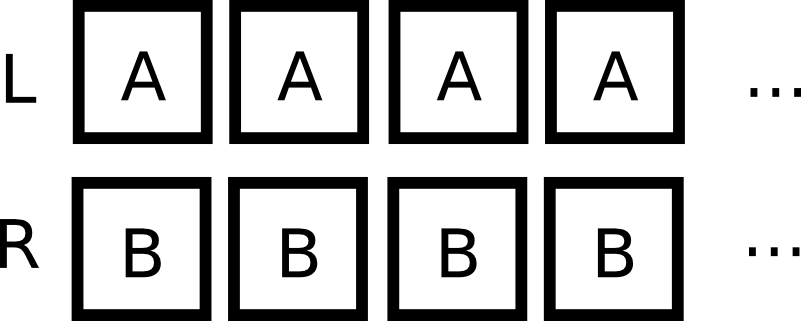
\includegraphics[width=2in]{pic/fmt-planar.png}}\;
  \subfloat[]{
\includegraphics[width=3in]{pic/fmt-interleaved.png}}
  \caption{Multi-channal data in planar (a) and interleaved (b) form.}
  \label{fig:interleaving}
\end{figure}

Another issue is the order in which the data from different semantic
channels is stored. We call a \emph{channel layout} a bijection $L : C
\rightarrow \mathbb{Z}_{\|C\|}$, where $C$ is a given \emph{channel
  space}. For example, the mapping $\{ left
\mapsto 0, right \mapsto 1 \}$ is a common layout for stereo sound,
but $\{ left \mapsto 1, right \mapsto 0 \}$ is sometimes used too.

\subsection{Common solutions}

As we have already noticed, 32 bit floating point sound with planar
left-right layout the most common in software of our kind during
internal processing. As most of this software is written in C, a
simple \texttt{float**} does the job. This was, actually, the internal
representation used in GNU Psychosynth in versions prior to 0.2.0,
wrapped in the \texttt{audio\_buffer} class.

However, this design starts to wobble whenever one has to interface
with some other library or hardware using a different format. Thus,
the \texttt{audio\_buffer} class provided different
\texttt{interleave\_*} and \texttt{deinterleave\_*}, where the
asterisk can be substituted by different sample formats like
\texttt{s16} or \texttt{s32} (fixed point signed 16 bit and 32 bit
respectively). This is very inconvenient because, as we have seen
through this section, many orthogonal factor affect audio
representation inducing a combinatorial explosion of format conversion
functions. Take a look at the 64 different read and write functions in
the \texttt{pcm.c} file of the
LibSndfile\footnote{\url{http://www.mega-nerd.com/libsndfile/}}
library.

This is a maintenance hell, but using the common means for abstracting
orthogonal behaviour variability, i.e. dynamic polymorphism, is simply
not an option in any audio software which supports real-time operation.

\subsection{A generic approach: Boost.GIL}

However, there is a piece of software that proved that this issue can be
solved in C++ using static polymorphism. This is the Generic
Image Library\footnote{http://stlab.adobe.com/gil} which was developed
by Ludovic Cortés et. Al inside Adobe Software Technology Lab that was
later include inside the Boost library distribution.

While sound and image manipulation are quite different, specially from
the psycho-perceptive point of view, they are both a signal processing
problem and thus share a lot in the representational issue. By
realising of a proper conceptual mapping between both worlds (table
\ref{tab:gilmap}), most of the library design and even quite a lot of
code of Boost.GIL can be reused to build a unique state-of-the-art
sound processing library that addresses the aforementioned issues in
an orthogonal generic manner while maintaining near-optimal
performance.

\begin{table}[h]
  \centering
  \begin{tabular}{c|c}
    Boost.GIL & Psynth.Sound \\ \hline\hline
    Channel   & Sample \\
    Color     & Channel \\
    Color Space & Channel Space \\
    Color Layout & Channel Layout \\
    Pixel & Frame \\
    View & Range \\
    Image & Buffer
  \end{tabular}
  \caption{Terminology map from \texttt{boost::gil} to \texttt{psynth::sound}}
  \label{tab:gilmap}
\end{table}

An \emph{image} is bidimensional matrix of \emph{pixels}, that capture
the properties of light electromagnetic waveform at those discrete
points. Each pixel, however, is decomposed in several \emph{colors}
that, for example, capture the intensity in the red, green and blue
sensors of a CCD camera. As there are different ways of decomposing an
audio frame (p.e, stereo, surround, etc.), there are different ways of
decomposing a pixel into several values, known as the \emph{color
  space} (p.e, RGB, CMYK, YUV, etc.). Boost.GIL uses the term
\emph{channel} to name the individual value of one those color
components.

In our audio framework, a \emph{buffer} is unidimensional array of
\emph{frames} that represent a sound or part of a sound --- sound is
continuous and thus we usually process it in chunks. The reader might
note that the the data in a buffer being arranged along the
\emph{time} dimension while the dimensions of an image represent
\emph{physical space} makes these entities completely different from
the processing point of view. However, they share most representation
problems, with sound representation being actually a sub-problem of
image representation, as we have one dimension less. The samples in a
series of audio frames can be stored in an interleaved or planar
fashion as happens with the channels of a pixel. Also, both channels
and samples can vary in signedness, fixed/floating point, bitdepth,
etc.

Those already familiar with Boost.GIL can thus already understand
easily our Psynth.Sound module design and implementation that we are
to describe in the following section.

\section{Design}

\subsection{Core techniques}

The Boost.GIL and thus the Psynth.Sound modules design makes heavy use
of static polymorphism and generic programming via C++ templates to
achieve generality without runtime overhead. We are going to introduce
advanced techniques used in generic programming for the reader
unfamiliar with this programming paradigm.

\subsubsection{Concepts}
\label{sec:concepts}.

\emph{Concepts} \cite{jarvi10concept} are to generic programming what
\emph{interfaces} --- pure abstract classes in C++ --- are to object
oriented programming: they specify the requirements on some
type. However there, are few substantial differences. (1) While
interfaces can only specify the method signatures of its instances, a
concept can specify most syntactic constraints on a type, like the
existence of free functions, operators, nested types, etc. (2) While
dispatching through interfaces requires, at least, a dereference,
addition and function call \cite{driesen96direct}, when using concepts
the concrete function to be executed can be determined and even
inlined at compile-time. (3) One can not declare that a type satisfies
an interface separately from the type definition, but one can say that
a type models a concept at any point of the program. (4) Thus, no
primitive type defines any virtual interface, but one can turn any
primitive type into an instance of any concept via a
\texttt{concept\_map}. (5) Actually, the syntactic properties defined
by a concept its models may differ, but they are matched via the
\texttt{concept\_map}. In fact, C++ concepts are more similar to
Haskell \emph{type classes}, with \texttt{instace} doing the job of
\texttt{concept\_map} \cite{bernardy08comparison}.

Concepts are an extension to the template mechanism to add type
checking for it. In fact, checking and dispatching on requirements can
be achieved with techniques like SFINAE (Substitution Failure Is Not
an Error) \cite{vandervoorde08templates}. Property (5) of our concepts
can be simulated with \emph{traits} \cite{c++traits}. However, both
compiler errors and the code using templates without concepts is
usually much more unreadable.

The proposal of adding concepts to the C++ language was rejected last
year by the standardisation committee and thus we can not use them in
our code. However, Boost.GIL is very influeced by Alexander Stepanov's
deductive approach to computer programming using generic programming
and modeling with concepts, that he elegantly describes in his
master-piece ``Elements of Programming''
\cite{stepanov09elements}. Actually Stepanov worked several years in
Adobe where he held a course ``Foundations of Programming'' based on
his book. Thus, the \emph{modeling} of the library extensively uses
concepts. Its implementation uses a limited form of concept checking
via the Boost.ConceptCheck\footnote{
  \url{http://www.boost.org/doc/libs/release/libs/concept_check/concept_check.htm}}
\cite{siek00concept} library, however, enabling this library in
release mode can affect performance and its syntax is quite more
cumbersome than the concepts in the C++ standard proposal. For
consistency with the Boost.GIL documentation we will use the concept
syntax proposed in the proposal N2081 to the standardisation committee
\cite{gregor06concept}.

The following example defines a concept that is satisfied by every
type that has an \texttt{operator<}:

\begin{lstlisting}
concept LessThanComparable<typename T> {
  bool operator< (T, T);
};
\end{lstlisting}

This allows us to write a generic function that depends on the
existence of a less-than comparator for the parametrised type:

\begin{lstlisting}
template<LessThanComparable T>
const T& min (const T& x, const T& y) {
  return x < y? x : y;
}
\end{lstlisting}

An alternative syntax for specifying that \texttt{T} must satisify the
\texttt{LessThanComparable} concept is the \texttt{where} clause:

\begin{lstlisting}
template<typename T>
    where LessThanComparable<T>
const T& min (const T& x, const T& y) ...
\end{lstlisting}

In fact, this is the only valid syntax when the concept affects
multiple types. Also, the \texttt{where} clause can be used inside
concept definitions to provide specialisation.

Specifying that a type models a concept is done with the
\texttt{concept\_map} device. If the type naturally models the
concept, we can just use:

\begin{lstlisting}
concept_map LessThanComparable<int> {}
\end{lstlisting}

Note that these trivial concept mappings can be avoided by using the
\texttt{auto} keyword in front of the \texttt{concept} keyword in the
concept definition. However, it might happen that a type requires some
wrapping to satisfy the concept. We can do this in the concept map
definition itself.

\begin{lstlisting}
concept_map LessThanComparable<char*> {
  bool operator< (char* a, char* b) {
    return strcmp (a, b) < 0;
  }
}
\end{lstlisting}

Note that this last piece of code is an example of a bad usage of
concept maps, as this specialises the mapping for pointers changing
the expected semantics.

This should suffice as an introduction to concepts in order to
understand the concept definitions that we will later show when
modelling our system. A more detailed view can be read in the cited
bibliography, with \cite{jarvi10concept} being the most updated and
useful from a programmer point of view.

\subsubsection{Metaprogramming}

The C++ template system is Turing complete
\cite{veldhuizen03templates}, thus it can be used to perform any
computation at \emph{compile time}. This was first noted in 1994 by
Erwin Unruh who, in the middle of a C++ standardisation committee,
wrote a template meta-program that outputted the first $N$ prime
numbers on the console using compiler errors \cite{unruh94prime}. Even
though this might seem just a crazy puzzle game, it can be used in
practise and actually new Boost libraries use it extensively. A very
gentle introduction to template metaprogramming can be found in
\cite{alexandrescu01modern}, where Alexandrescu uses them to
instantiate design patterns as generic C++ libraries. A deeper
reference is Abraham's \cite{abrahams04meta}, which focuses on the
Boost Metaprogramming Library\footnote{The Boost.MPL:
  www.boost.org/doc/libs/release/libs/mpl} and introduces the usage of
metaprogramming for building Embedded Domain Specific Languages (EDSL)
in C++. This Boost.MPL, providing reusable meta data structures and
algorithms, is the de-facto standard library for template
metaprogramming\footnote{It is often called ``the STL of template
  metaprogramming''.} and we will use it in our implementation.

Template metaprogramming is possible thanks to \emph{partial template
  specialisation}, that allows giving an alternate definition for a
pattern matched subset of its possible parameter values. A
\emph{metafunction} is thus just a template \texttt{class} or
\texttt{struct} with a public member that holds the result of the
function. It is up to the programmer to choose the naming convention
for the result members of the metafunctions, in the following, we will
use Abraham's style calling \texttt{type} for result values that are a
type, and \texttt{value} for integral values. Listing \ref{lst:fib}
illustrates how can we write and use a metafunction for computing the
$n$-th Fibonacci number.

\begin{lstlisting}[float=h!, 
  caption=Metaprogram for computing the Nth Fibonacci number,
  label=lst:fib]
template <int N>
struct fib {
  enum { 
    value = fib<N-1>::value + fib<N-2>::value; 
  };
};

template <>
struct fib <0> {
  enum { value = 0 };
};

template <>
struct fib <1> {
  enum { value = 1 };
};

int main () {
  return fib<42>::value;
}  
\end{lstlisting}

The program returns the forty-second Fibonacci value. However, it will
take no time to execute, because the number is computed at compile
time. We use recursion to define the metafunction for the general case
and the specialise for the base cases.

If we consider the template system as a meta-language on its own, we
should describe its most outstanding semantic properties. It is a pure
functional programming language, because variables are immutable. It
is lexically scoped. It supports both lazy and strict evaluation,
depending on whether we choose to access the nested \texttt{type}
result name at call site or value usage type. When we look at the meta
type system, we find three meta types: types (which are duck-typed
records), integrals (e.g. \texttt{int}, \texttt{char}, \texttt{bool}
...) and meta-functions (i.e. templates).

The fact that records are duck typed but integrals and metafunctions
cause several inconveniences in practice, specially when dealing with
the later. For example, in the absence of template aliases, returning
a metafunction produced by another function requires defining a nested
struct that inherits from the actual synthesised value. Also, the
template signature should be specified on a template parameter
expecting a template.

In order to simplify our meta type system we shall wrap constants in a
type like on listing \ref{lst:integral_c}.

\begin{lstlisting}[float, 
  caption=Integral constant nullary metafunction  wrapper.,
  label=lst:integral_c]
template <typename T, T V>
struct integral_c
{
  BOOST_STATIC_CONSTANT(T, value = V);
  typedef integral_c<T, V> type;
};
\end{lstlisting}

There are a couple of issues regarding this definition worth
explaining. First, the \texttt{BOOST\_STATIC\_CONSTANT} macro is used
to define a constant. Internally, it will try to use \texttt{enum} or
any other mechanism available to actually define the constant such
that the compiler is not tempted to allocate static memory for the
constant. Second, the \texttt{typedef} referring to itself turns a
constant value into a self returning nullary meta-function. This can
be very convenient because, for example, it allows using
\emph{value}\texttt{::type::value} always on the value usage point,
allowing the caller or producer of the value to choose whether he
wants to evaluate the value lazily.

Because we just wrapped values into a type, we can simplify our
conventional definition of \emph{metafunction}: a meta-function is any
type --- template or not --- that has a nested type called
\texttt{type}.

Now we should also turn metafunctions into first class entities of the
meta-language. We just add a new level of indirection and define a
\emph{metafunction class} as a type with a nested template
metafunction called \texttt{apply}. The example in listing
\ref{lst:high_order_fib} also illustrates the metafunction forwarding
technique when defining the nested \texttt{apply} metafunction by
inheriting from \texttt{fib}.

\begin{lstlisting}[float, caption=Metafunction class for
  computing Fibonacci numbers. We suppose that the previous
  \texttt{fib} definition uses \texttt{integral\_c} to wrap its
  parameters and return types., label=lst:high_order_fib]
struct fib_class { 
   template <class N>
   struct apply : public fib<N> {};
};

int maint ()
{
  return fib_class::apply<integral_c<int, 42>>
           ::type::value;
}
\end{lstlisting}

Using this convention the MPL library defines many useful high order
metafunctions that take metafunction classes as input, like
\texttt{mpl::fold} and \texttt{mpl::transform}. Note that it is not
needed to define metafunction classes for all our metafunctions,
instead, we shall convert them when needed using the
\texttt{mpl::quote}\emph{N} functions and the \texttt{mpl::lambda}
facility.

\subsection{Core concepts}

We are now ready to understand the main design and implementation
techniques used in our generic library. Because the library is
\emph{generic}, in the sense of generic programming, most algorithms
and data structures are parametrised such that they can be
instantiated with any concrete type modelling some concepts as we
suggested in section \ref{sec:concepts}. Thus, traditional modelling
techniques like the Unified Modelling Language are not useful since
they are intended for object oriented design.

We are going to follow the following methodology for describing the
library. First, we will name a concept and give a brief description of
its purpose. Then, we will define the concept using the notation
described in section \ref{sec:concepts} and finally we will enumerate
and describe some models for such concept.

For brevity, we will omit basic concepts such as
\texttt{CopyConstructible}, \texttt{Regular}, \texttt{Metafunction},
etc. Their complete definition should be evident and an interested
reader can find most of them in \cite{stepanov09elements}.

\subsubsection{\texttt{ChannelSpaceConcept}}

A channel space is a sequence of whose elements channel tags (empty
types giving a name )

\begin{lstlisting}
concept ChannelSpaceConcept<
           MPLRandomAccessSequence Cs> 
{};
\end{lstlisting}

Some example models include \texttt{stereo\_space} or
\texttt{surround\_space}. An example on how a user of the library can
define his own channel space follows.

\begin{lstlisting}
struct left_channel;
struct right_channel;

typedef mpl::vector<left_channel, right_channel> 
        stereo_space;
\end{lstlisting}


\section{Validation}


%%% Local Variables: 
%%% mode: latex
%%% TeX-master: "00-main"
%%% End: 
